\documentclass[11pt,letterpaper,twoside]{article}
\usepackage[english]{babel}
\usepackage{amssymb,amsmath}
\usepackage{fancyhdr}
\usepackage{graphicx}

 \oddsidemargin  0in \evensidemargin 0in
 \topmargin   -0.25in \headheight 0.25in \headsep 0.25in
 \textwidth   6.5in \textheight 8.75in \marginparsep 0pt \marginparwidth 0pt
 \parskip 1ex  \parindent 0ex \footskip 20pt

\newfont{\bssten}{cmssbx10}
\newfont{\bssnine}{cmssbx10 scaled 900}

%%%%%%%%%%%%%%%%%%%%%%%
\newcommand{\whatizit}{Lecture 11: Random Variables}
%%%%%%%%%%%%%%%%%%%%%%%


\pagestyle{fancy}  
\fancyhead{\bssnine STOR 155,  \whatizit}
\fancyhead[RE]{} \fancyhead[LO]{}
\fancyhead[LE]{\bssnine \thepage} \fancyhead[RO]{\bssnine \thepage}
\lfoot{} \cfoot{} \rfoot{}   


\newcommand{\var}{\mathrm{Var}}



\begin{document}



\thispagestyle{empty} \vspace*{-0.75in}

{\bssten STOR 155: Introduction to Data Models and Inference \hfill May 30, 2024 \\
Prof. Will Lassiter  \hfill Page 1 of \pageref{totalpag}}
\vspace{10pt}
\begin{center} {{\Large \bf \whatizit}} \end{center}

{\bf Definition and Types} \vspace{6pt}

A {\bf random variable} is ... \vspace{40pt}

Examples: \vspace{240pt}

Two major types of random variables:

\begin{enumerate}

\item \quad

\vspace{100pt}

\item \quad

\end{enumerate}

\newpage

Discrete random variables: two examples \vspace{6pt}

Let $X$ represent \vspace{40pt}

\begin{center}
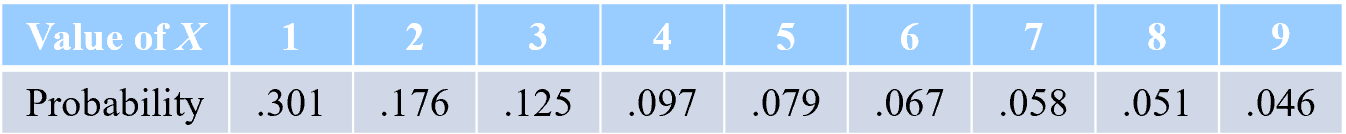
\includegraphics[scale=0.9]{images/benford.png}
\end{center}

Let $Y$ represent \vspace{40pt}

\begin{center}
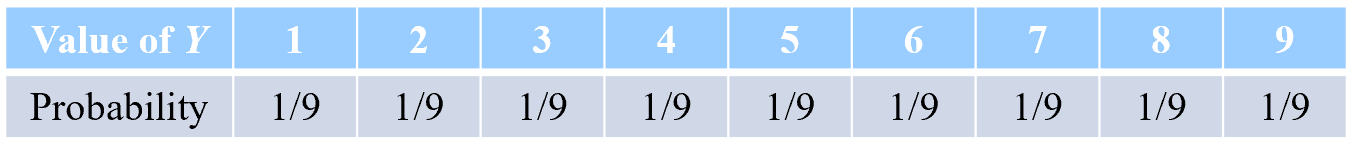
\includegraphics[scale=0.9]{images/randbetween.png}
\end{center}

\vspace{80pt}

Continuous random variables: one example \vspace{6pt}

Let $H$ represent \vspace{40pt}

\begin{center}
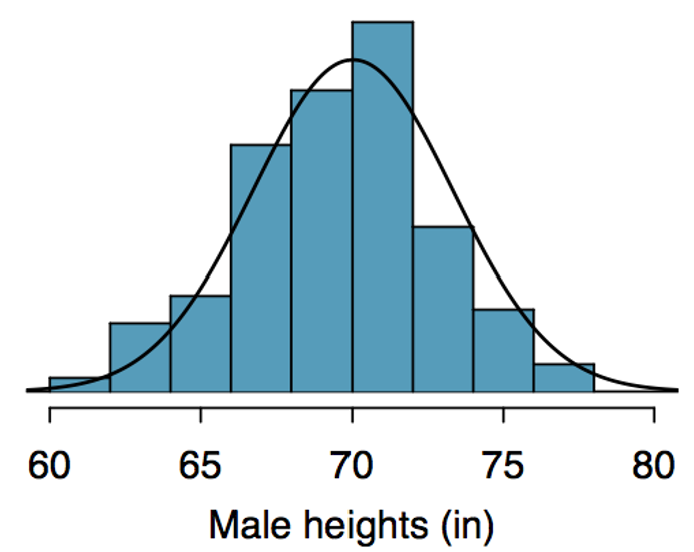
\includegraphics[scale=0.9]{images/density.png}
\end{center}

\newpage

{\bf Mean and Variance for Discrete Random Variables} \vspace{6pt}

Example: bookstore revenue \vspace{60pt}

\begin{center}
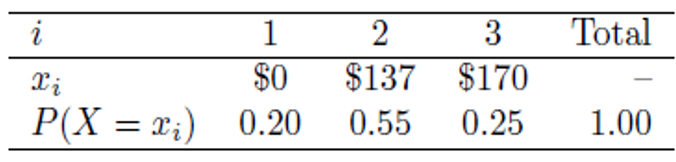
\includegraphics[scale=0.9]{images/bookstore.png}
\end{center}

\vspace{120pt}

{\bf Mean} or {\bf expected value} of a discrete random variable: \vspace{165pt}

\begin{center}
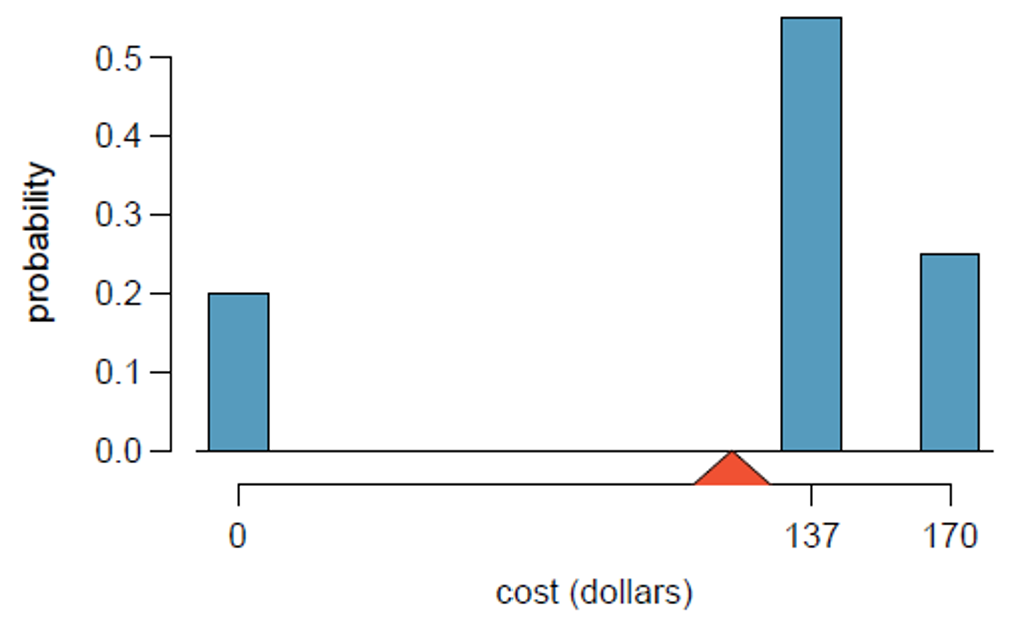
\includegraphics[scale=0.6]{images/bookstore2.png}
\end{center}

\newpage

Random phenomenon: Bet \$1 on a game of Chuck-a-Luck (casino dice game) and let $X$ represent your net gain or loss from that bet. 

\begin{center}
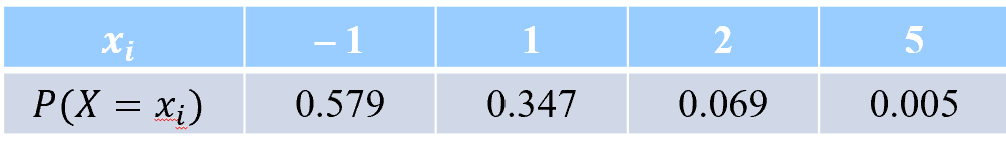
\includegraphics[scale=0.8]{images/chuck.png}
\end{center}

Expected gain/loss is: \vspace{40pt}

Interpretation: \vspace{150pt}

Random phenomenon: Take a SRS of size 3 from a large population that is $\frac{2}{3}$ female, $\frac{1}{3}$ male, and let $X$ represent the number of females in the sample.

\begin{center}
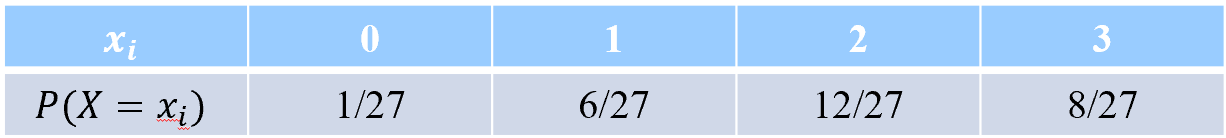
\includegraphics[scale=0.7]{images/srs.png}
\end{center}

Calculate $E[X]$.

\newpage

Bookstore example revisited:

\begin{center}
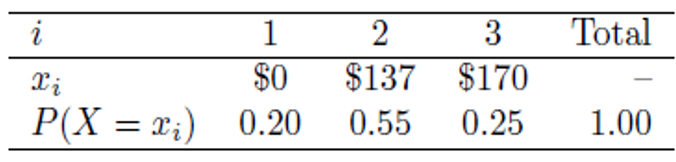
\includegraphics[scale=0.9]{images/bookstore.png}
\end{center}

\vspace{30pt}

{\bf Variance} of a discrete random variable: \vspace{150pt}

Rules for mean and variance: example \vspace{10pt}

\begin{center}
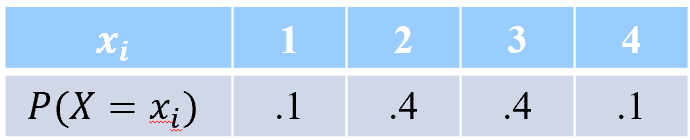
\includegraphics[scale=0.8]{images/x.png}\hspace{20pt} 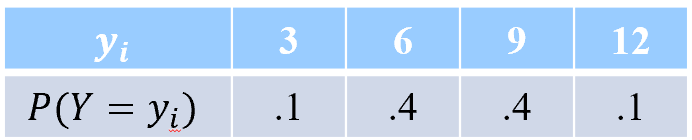
\includegraphics[scale=0.8]{images/y.png}
\end{center}

\begin{center}

\end{center}

\newpage

Rules for mean and variance:  For random variables $X$ and $Y$ and constants $a$ and $b$, \vspace{300pt}

Random phenomenon: Roll 2 ``weird" 6-sided dice: one has faces with 1,3,4,5,6,8 pips; the other has faces with 1,2,2,3,3,4 pips. Let $Z$ be the total number of pips on the two up-faces. \vspace{150pt}

Random phenomenon: Toss a fair coin 4 times, and let $X$ be the number of flips that come up heads and $Y$ the number of flips that come up tails.

\newpage

One more rule for variance: \vspace{100pt}

Random phenomenon: My commute to work takes $X$ minutes, where $X$ is a random variable with mean 15 minutes and standard deviation 2 minutes.  The same is true for my commute back home.

\begin{itemize}

\item Mean and variance of my total commute time in a day? \vspace{100pt}

\item Mean and variance of my total commute time in a workweek (5 days)? \vspace{100pt}

\end{itemize}

Example: A mechanical assembly consists of a rod with a bearing on each end. The three parts are manufactured independently, and all vary a bit from part to part. Rods have mean length 12 cm and st.\ dev.\ 4 mm. Bearings have mean length 2 cm and st.\ dev.\ 4 mm.

\begin{center}
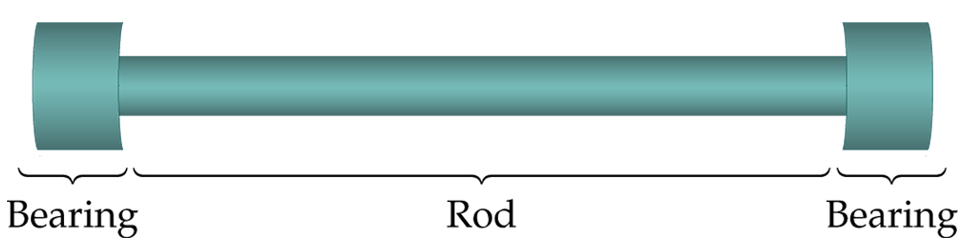
\includegraphics[scale=0.6]{images/assembly.png}
\end{center}

What are the mean and st.\ dev.\ of the total length of the assembly?

\label{totalpag}
\end{document}